% Created 2010-08-17 Tue 13:49
\documentclass{article}
\usepackage{graphicx}
\usepackage{times}
\usepackage[margin=0.75in]{geometry}


\title{Inserting an AHIR module in the NetFPGA framework}
\author{Madhav Desai}

\begin{document}

\maketitle

\section{Overview}

This document describes the mechanism by which an 
AHIR generated VHDL system can be included in the NetFPGA packet
processing implementation framework.  

The AHIR generated VHDL system is required to fit into 
a NetFPGA user-module template. It is relatively easy to
achieve this. 


\section{Mechanism}

The user module template has the form shown in Figure \ref{fig:NetFPGAUserModule}.
\begin{figure}
  \centering
  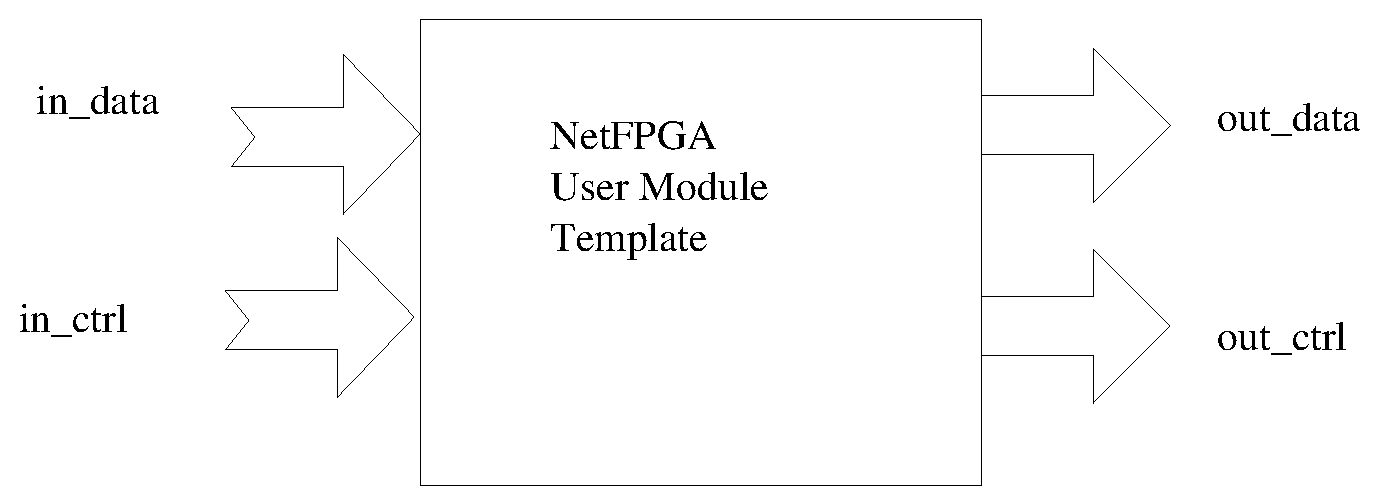
\includegraphics[scale=0.7]{NetFPGAUserModule.eps}
  \caption{NetFPGA User Module}
  \label{fig:NetFPGAUserModule}
\end{figure}
The interface is very simple: an input data and control bus,
and an output data and control bus.

A generic AHIR system can have the form:
\begin{figure}
  \centering
  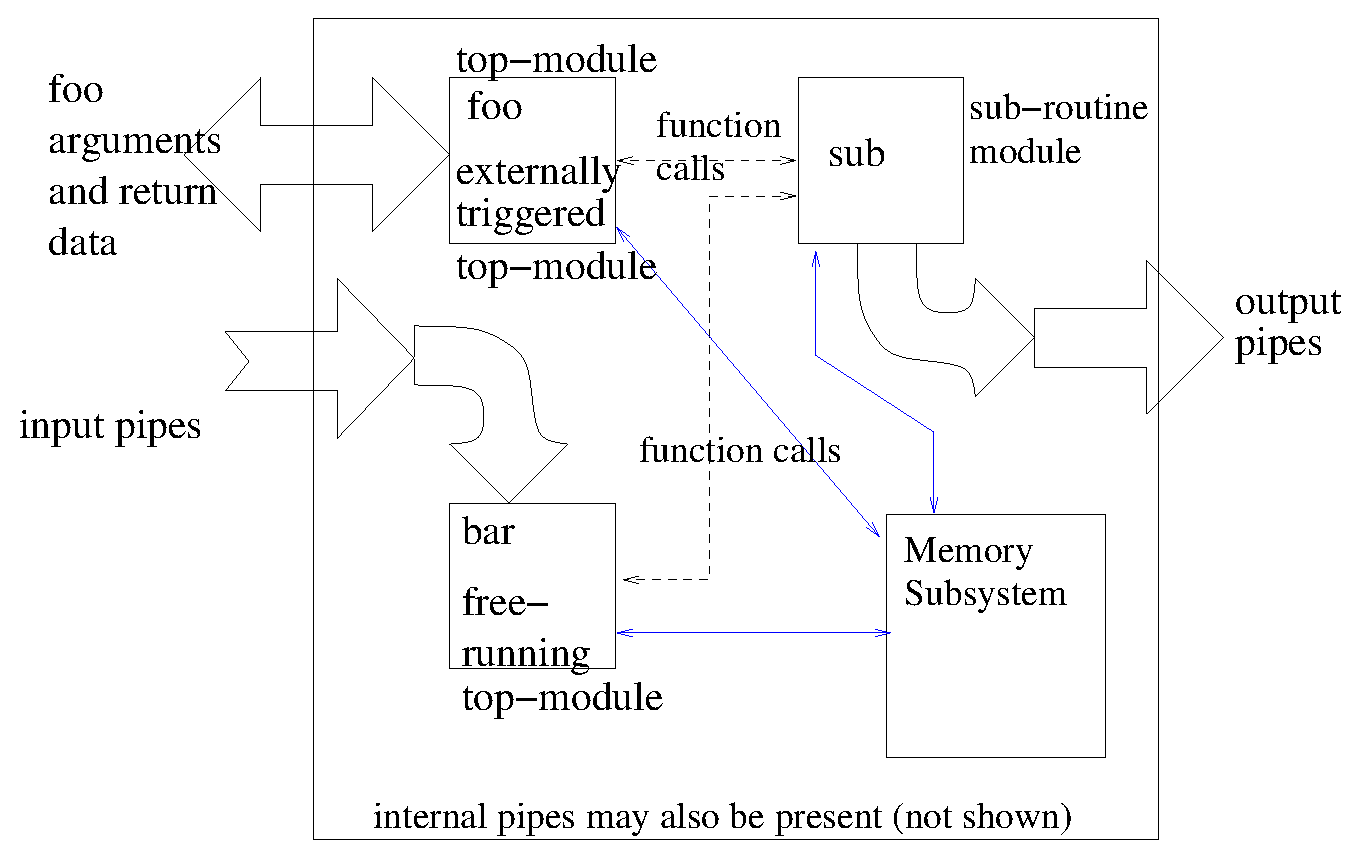
\includegraphics[scale=0.7]{GenericAhirSystem.eps}
  \caption{Generic AHIR system}
  \label{fig:GenericAhirSystem}
\end{figure}



Thus, in order to insert a generic AHIR system into a NetFPGA user-module template:
\begin{itemize}
\item we ensure that the only interaction of the AHIR system with the outside world is
through four pipes: two input pipes for the input data and control, and
two output pipes for the output data and control.
\item The top-level modules in the AHIR system are free-running.  One solution
would be to include two top-level free-running modules which are 
responsible for interactions with the outside world (through the four pipes
discussed above).
\begin{itemize}
\item an input-module which will collect data from the input pipes and
forward to appropriate pipes/modules in the AHIR system.
\item an output-module which will collect data from internal pipes/modules
in the AHIR system and forward it to the the system output pipes.
\end{itemize}
\item The AHIR system would be instantiated in a {\em fixed} wrapper
which would be responsible for the protocol matching between the AHIR
system interface and the NetFPGA user module interface.
\end{itemize}


\section{Issues: memory management}

One issue that needs to be resolved is that of memory management.
This relates to two processes:
\begin{itemize}
\item Initialization: if the memory subsystem in the AHIR module needs
to be initialized, then this must be done explicitly by the outside
world.  The llvm2aa tool can generate memory initialization modules
that initialize the data structures in the system to their initial
values as declared in the original C program.  These modules are
auto-generated and need to be called once after the AHIR system
is reset (this call-once feature can be incorporated into vc2vhdl).
\item Exchange of information between the AHIR memory subsystem and
the outside world:  If this is needed, it would need to be explicitly 
built into the input/output modules.  Note that an exchange of
information (in general) may be initiated from ``inside'' or
from ``outside'' the AHIR system.
\end{itemize}

\section{Proposal}

The process of including the AHIR system in a NetFPGA user template is
exactly the same as that of verifying an AHIR system using a C-testbench
with the assumption that the testbench only sends/receives packets to the AHIR 
system.  Most of the basic infrastructure for this is in place.  The only
necessary components are the input and output modules outlined in the 
previous section.

Originally, Sameer had implemented the input and output module for
a specific scenario (as documented in the previous plan).  In this
scenario, the input module would receive the data from the NetFPGA
surroundings, would put the data packet into memory and would trigger
the AHIR module.  On completion of the AHIR module, the output module
would take the modified data from memory and would forward it to
the NetFPGA environment.   I have looked at the code and it
seems reasonably clean (will probably have to redo parts of it
to fit into the new AhirV2 scheme). 

What would be easiest, in my opinion would be
\begin{itemize}
\item use the parts of Sameer's code that do the protocol
translation (between the NetFPGA user-module and an AHIR module).
\begin{itemize}
\item we implement a VHDL entity {\em NetFpgaAhirSystemWrap} which 
would instantiate an AHIR system with four interface pipes (see Figure \ref{fig:NetFpgaAhirSystemWrap}).
\begin{figure}
  \centering
  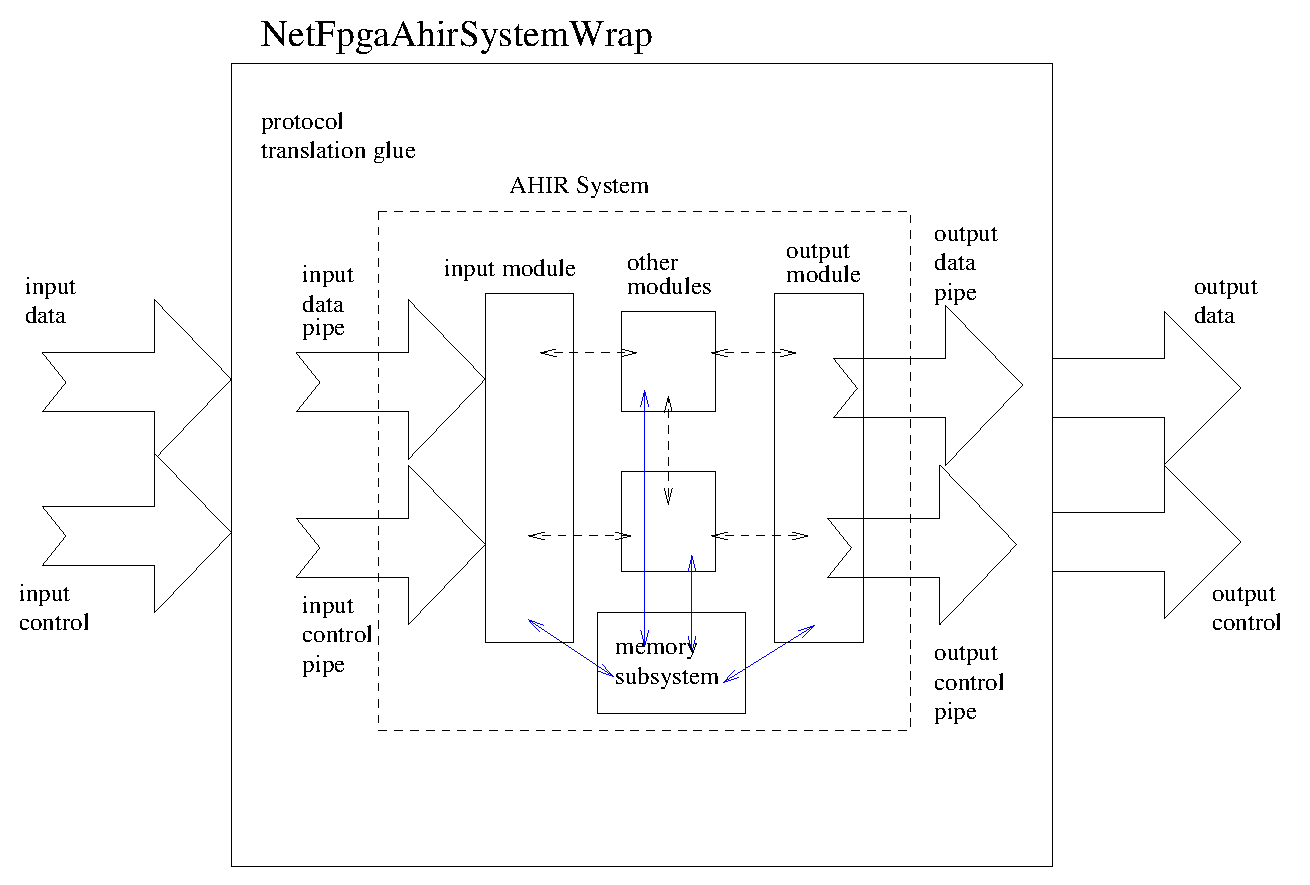
\includegraphics[scale=0.7]{NetFpgaAhirSystemWrap.eps}
  \caption{NetFpgaAhirSystemWrap Schematic}
  \label{fig:NetFpgaAhirSystemWrap}
\end{figure}
\end{itemize}
\item write the input and output modules in C/Aa and add
to the AHIR flow to generate the final system. 
\begin{itemize}
\item this can be user-written (and eventually auto-generated) for
the specific system being generated.  Note that we will have
to pay some attention to memory initialization and transfer of
information between the AHIR memory subsystem and the outside
world.
\end{itemize}
\item generate the final AHIR system by including the input/output modules
written in C/Aa.
\item Instantiate the final AHIR system in the NetFpgaAhirSystemWrap wrapper.
\end{itemize}
The process is indicated in Figure \ref{fig:Wrap}.   The only
additional effort is to write the input and output modules (in C or Aa).


\begin{figure}
  \centering
  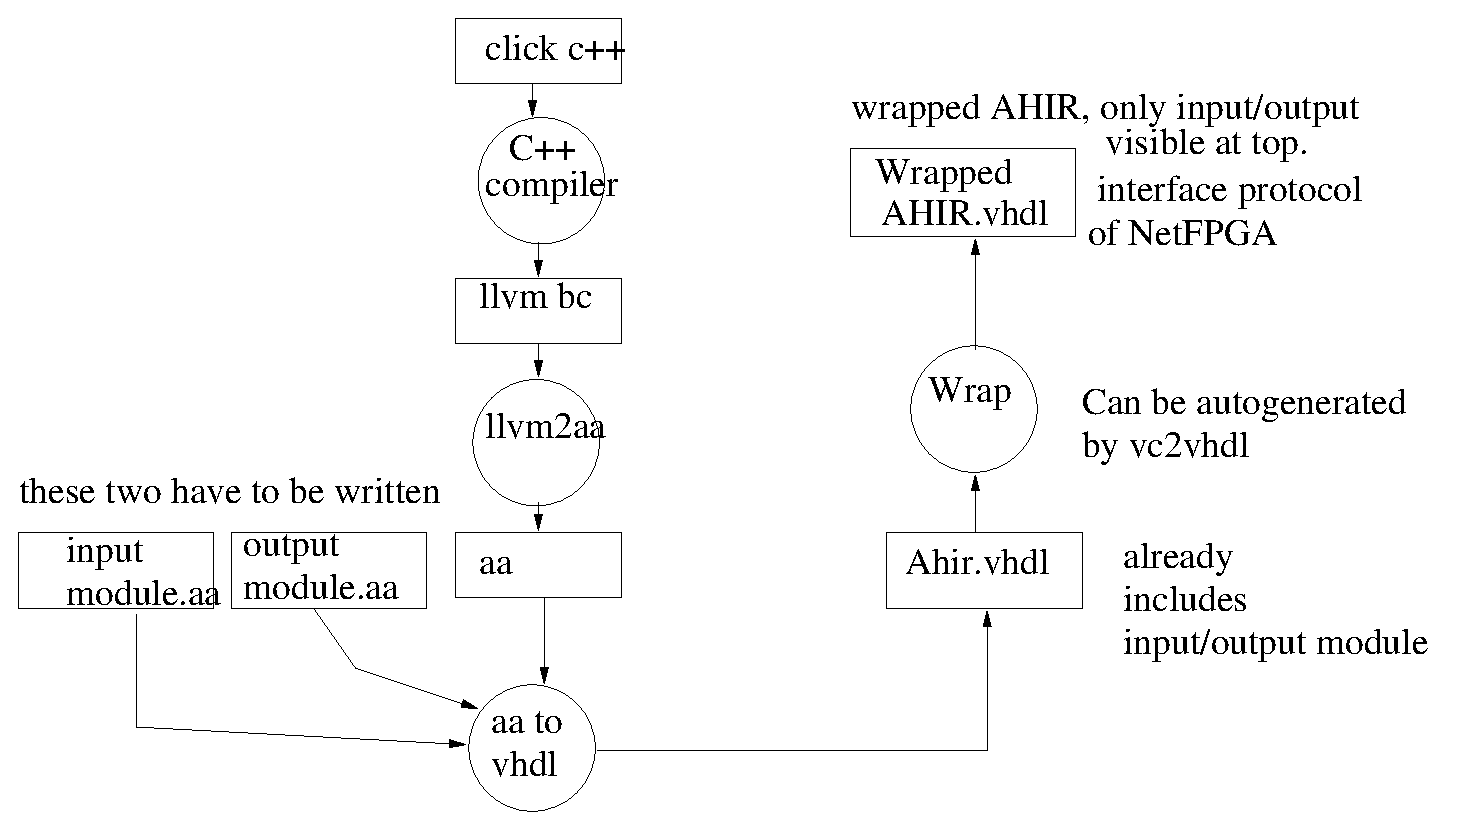
\includegraphics[scale=0.7]{NetFPGAWrap.eps}
  \caption{NetFPGA Wrap Flow}
  \label{fig:Wrap}
\end{figure}

\section{NetFPGA Wrapper Module}




\end{document}
